\documentclass[11pt,a4paper]{article}

\usepackage[utf8]{inputenc}
\usepackage[T1]{fontenc}
\usepackage{lmodern}
\usepackage{microtype}
\usepackage[margin=0.92in]{geometry}
\usepackage{amsmath,amssymb,amsfonts}
\usepackage{booktabs}
\usepackage{float}
\usepackage{xcolor}
\usepackage{hyperref}
\usepackage{enumitem}
\usepackage{caption}
\usepackage{tikz}
\usepackage{pgfplots}
\usepackage[most]{tcolorbox}
\usetikzlibrary{positioning,arrows.meta,calc}
\pgfplotsset{compat=1.16}
\linespread{1.07}

\definecolor{amblue}{HTML}{2563EB}
\definecolor{amgreen}{HTML}{16A34A}
\definecolor{amteal}{HTML}{0D9488}
\definecolor{amgray}{HTML}{64748B}
\definecolor{amred}{HTML}{DC2626}
\definecolor{amorange}{HTML}{EA580C}
\definecolor{codebg}{HTML}{F8FAFC}

\hypersetup{
  colorlinks=true,
  linkcolor=amblue,
  urlcolor=amblue,
  pdftitle={Giving AI Assistants a Reliable Notebook: How Agent Memory Works Under the Hood},
  pdfauthor={Dorian Herle}
}
\captionsetup{font=small,labelfont=bf}
\setlength{\parskip}{0.5em}
\setlength{\parindent}{0pt}

\newtcolorbox{callout}[1][]{colback=blue!4,colframe=amblue,fonttitle=\bfseries,title=#1,boxrule=0.6pt,arc=3pt}
\newtcolorbox{mathbox}[1][]{colback=gray!4,colframe=gray!45,fonttitle=\bfseries\small,title=#1,boxrule=0.5pt,arc=3pt}
\newtcolorbox{glossarybox}{colback=gray!6,colframe=gray!50,boxrule=0.5pt,arc=3pt,fontupper=\small}

\title{\textbf{Giving AI Assistants a Reliable Notebook}\\[4pt]\large How Agent Memory keeps track of long, multi-day work---in plain words and concrete math}
\author{\textbf{Dorian Herle}\\\texttt{herle.dorian@gmail.com}\\\small\url{https://github.com/dorianherle/agent_memory}}
\date{October 14, 2026}

\begin{document}
\maketitle

% ---------------------------------------------------------------
\begin{callout}[The short version]
AI assistants are increasingly asked to do work that spans many sessions, such as building software or working through a multi-step mathematical derivation. Yet each new session starts with a blank mind. Existing fixes either dump the entire past transcript into the prompt (which buries key facts and explodes in cost) or \emph{summarize and slice} old notes (which destroys exact equations and code constants).

We built \textbf{Agent Memory}, which works like a well-kept engineering notebook: it saves whole notes with Git file snapshots, hands the assistant a deterministic \textbf{1{,}200-character cheat sheet} at the start of every turn (with zero extra AI calls), folds completed steps together, and lets the assistant pull up uncut pages in a single lookup when needed. On the ICML 2026 \emph{MemoryArena} physics benchmark (20 papers, 86 steps), it kept \textbf{100\% of needed equations intact} and helped a strong AI model finish \textbf{all 20 multi-step problems (86/86 steps)}, compared with 7 out of 20 without memory.
\end{callout}

% ---------------------------------------------------------------
\section{The problem: a colleague who forgets every morning}

Imagine a brilliant colleague who gets amnesia overnight. On Monday you explain the setup of a project and derive a key formula. On Wednesday you ask them to apply Monday's formula to a new case. They remember nothing.

That is how AI assistants work across sessions today. To bridge the gap, people attach an external memory system. The three standard approaches all break down on technical work:

\begin{itemize}[itemsep=2pt,leftmargin=1.5em]
  \item \textbf{Hand over the whole transcript (Long Context).} Nothing is thrown away, but after $k$ sessions the prompt contains every dead end, wrong turn, and verbose tool log. Important definitions get drowned out, and token cost grows quadratically ($\mathcal{O}(k^2)$).
  \item \textbf{Keep short AI-written summaries (e.g., Mem0).} An auxiliary AI rewrites each session into short bullet points like \emph{``established a locality rule for the amplitude.''} In technical work, the exact number or sign ($\sigma = 4$, $c_2 = -1$) is the very thing that gets paraphrased away.
  \item \textbf{Search the transcript in fixed-size slices (Chunk RAG / BM25).} The transcript is chopped every 400--500 characters. A definition at the top of a page and the equation at the bottom end up in separate slices, so searching retrieves one without the other (Figure~\ref{fig:problem}).
\end{itemize}

\begin{figure}[H]
\centering
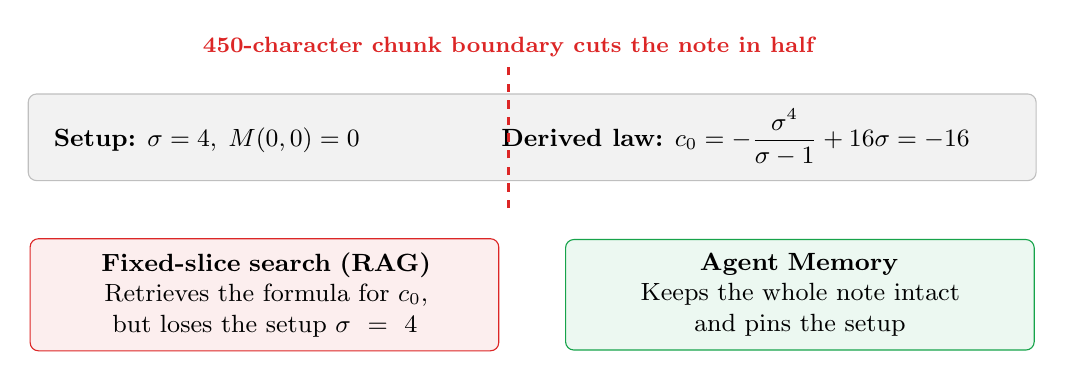
\begin{tikzpicture}[font=\small]
  \draw[rounded corners=3pt,fill=gray!10,draw=gray!50] (0,0) rectangle (12.8,1.1);
  \node[anchor=west] at (0.2,0.55) {\textbf{Setup:} $\sigma = 4,\; M(0,0)=0$\hspace{1.8cm}\textbf{Derived law:} $c_0 = -\dfrac{\sigma^4}{\sigma-1} + 16\sigma = -16$};
  \draw[amred,very thick,dashed] (6.1,-0.35) -- (6.1,1.45);
  \node[amred,font=\footnotesize\bfseries] at (6.1,1.7) {450-character chunk boundary cuts the note in half};
  \node[draw=amred,fill=amred!8,rounded corners=3pt,align=center,text width=5.6cm,inner sep=5pt] at (3.0,-1.45)
    {\textbf{Fixed-slice search (RAG)}\\ Retrieves the formula for $c_0$, but loses the setup $\sigma=4$};
  \node[draw=amgreen,fill=amgreen!8,rounded corners=3pt,align=center,text width=5.6cm,inner sep=5pt] at (9.8,-1.45)
    {\textbf{Agent Memory}\\ Keeps the whole note intact\\ and pins the setup};
\end{tikzpicture}
\caption{Why fixed-size chunking fails on math and code: slicing text every few hundred characters separates a formula from the definitions required to evaluate it.}
\label{fig:problem}
\end{figure}

% ---------------------------------------------------------------
\section{How Agent Memory works: step-by-step schematic and concrete math}

Scientists and engineers solved this problem long ago with a structured lab notebook: write complete entries, track when files change, read a one-paragraph status summary each morning, and flip to the full page when you need a detailed derivation. Agent Memory turns those habits into a deterministic six-step pipeline (Figure~\ref{fig:loop}).

\begin{figure}[H]
\centering
\makebox[\textwidth][c]{%
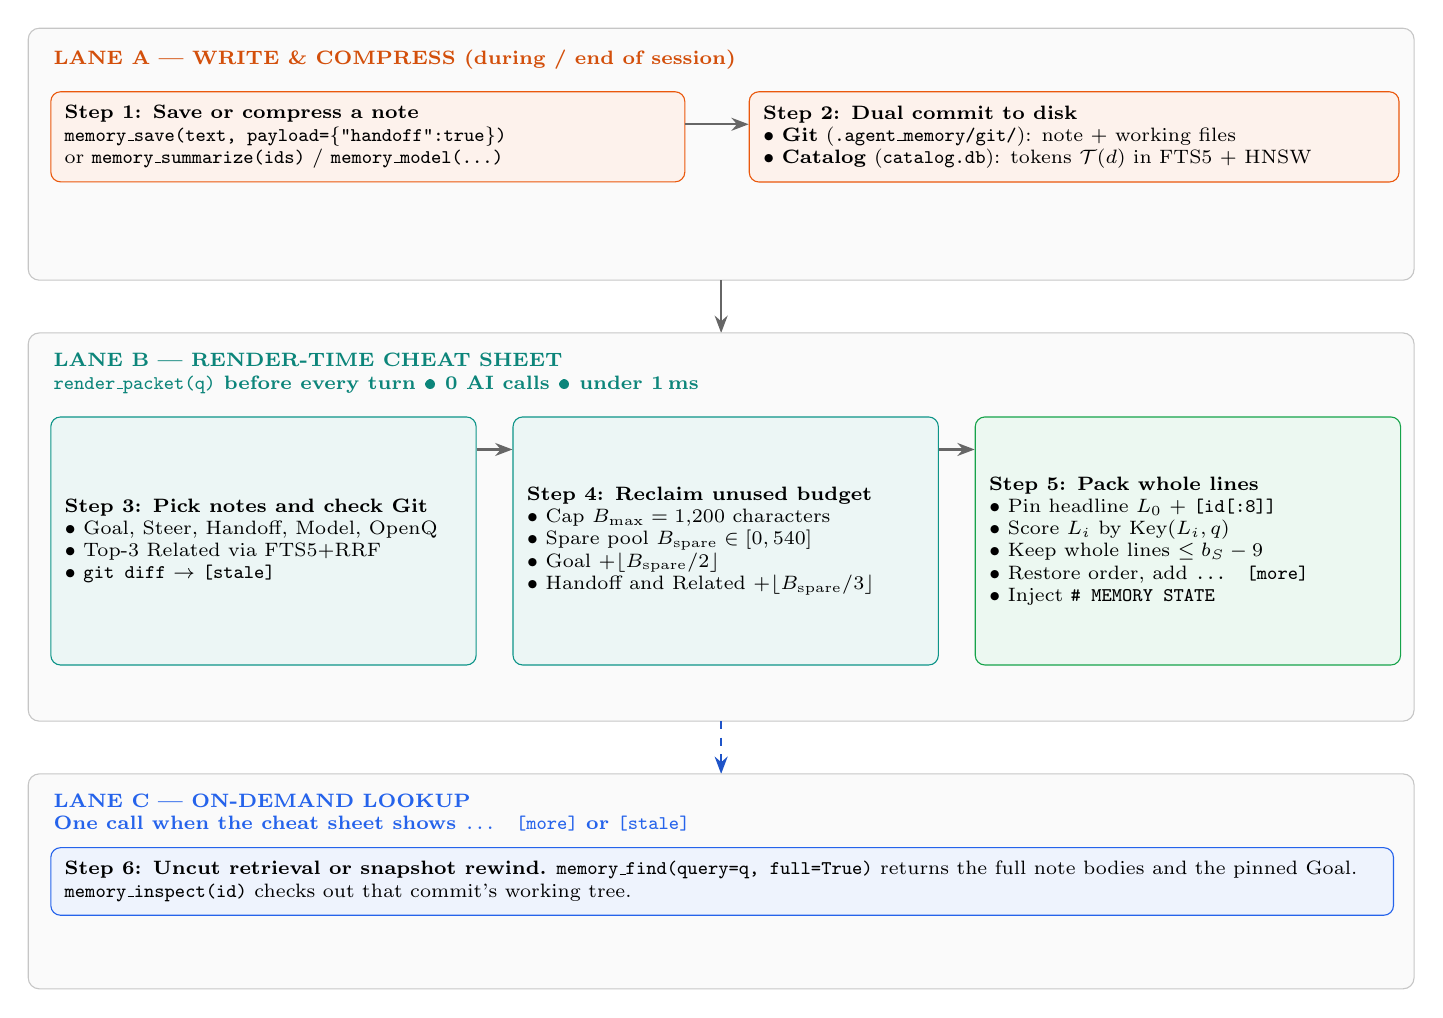
\begin{tikzpicture}[
  box/.style={draw,rounded corners=3.5pt,align=flush left,inner sep=5pt,font=\scriptsize},
  lane/.style={draw=gray!45,fill=gray!4,rounded corners=4pt},
  hd/.style={anchor=north west,font=\scriptsize\bfseries,inner sep=1pt,align=flush left},
  arr/.style={-{Stealth[length=2.2mm]},thick,gray!80!black}]

  % Lane A. Arrows stay in the gaps between cards and between lanes.
  \draw[lane] (0,9.15) rectangle (17.6,12.35);
  \node[hd,text=amorange!90!black] at (0.28,12.12)
    {LANE A --- WRITE \& COMPRESS (during / end of session)};
  \node[box,fill=amorange!8,draw=amorange,text width=7.7cm,anchor=north west] (w1) at (0.28,11.55)
    {\textbf{Step 1: Save or compress a note}\\
     \texttt{memory\_save(text, payload=\{"handoff":true\})}\\
     or \texttt{memory\_summarize(ids)} / \texttt{memory\_model(...)}};
  \node[box,fill=amorange!8,draw=amorange,text width=7.9cm,anchor=north west] (w2) at (9.15,11.55)
    {\textbf{Step 2: Dual commit to disk}\\
     $\bullet$ \textbf{Git} (\texttt{.agent\_memory/git/}): note + working files\\
     $\bullet$ \textbf{Catalog} (\texttt{catalog.db}): tokens $\mathcal{T}(d)$ in FTS5 + HNSW};
  \draw[arr] ($(w1.north east)+(0,-0.42)$) -- ($(w2.north west)+(0,-0.42)$);
  \draw[arr] (8.8,9.15) -- (8.8,8.48);

  % Lane B
  \draw[lane] (0,3.55) rectangle (17.6,8.48);
  \node[hd,text=amteal!90!black] at (0.28,8.26)
    {LANE B --- RENDER-TIME CHEAT SHEET\\
     \texttt{render\_packet(q)} before every turn \textbullet\ 0 AI calls \textbullet\ under 1\,ms};
  \node[box,fill=amteal!8,draw=amteal,text width=5.05cm,minimum height=3.15cm,anchor=north west] (r1) at (0.28,7.42)
    {\textbf{Step 3: Pick notes and check Git}\\
     $\bullet$ Goal, Steer, Handoff, Model, OpenQ\\
     $\bullet$ Top-3 Related via FTS5+RRF\\
     $\bullet$ \texttt{git diff} $\to$ \texttt{[stale]}};
  \node[box,fill=amteal!8,draw=amteal,text width=5.05cm,minimum height=3.15cm,anchor=north west] (r2) at (6.15,7.42)
    {\textbf{Step 4: Reclaim unused budget}\\
     $\bullet$ Cap $B_{\max}=1{,}200$ characters\\
     $\bullet$ Spare pool $B_{\text{spare}}\in[0,540]$\\
     $\bullet$ Goal $+\lfloor B_{\text{spare}}/2\rfloor$\\
     $\bullet$ Handoff and Related $+\lfloor B_{\text{spare}}/3\rfloor$};
  \node[box,fill=amgreen!8,draw=amgreen,text width=5.05cm,minimum height=3.15cm,anchor=north west] (r3) at (12.02,7.42)
    {\textbf{Step 5: Pack whole lines}\\
     $\bullet$ Pin headline $L_0$ + \texttt{[id[:8]]}\\
     $\bullet$ Score $L_i$ by $\text{Key}(L_i,q)$\\
     $\bullet$ Keep whole lines $\le b_S-9$\\
     $\bullet$ Restore order, add \texttt{... [more]}\\
     $\bullet$ Inject \texttt{\# MEMORY STATE}};
  \draw[arr] ($(r1.north east)+(0,-0.42)$) -- ($(r2.north west)+(0,-0.42)$);
  \draw[arr] ($(r2.north east)+(0,-0.42)$) -- ($(r3.north west)+(0,-0.42)$);
  \draw[arr,dashed,amblue!85!black] (8.8,3.55) -- (8.8,2.88);

  % Lane C
  \draw[lane] (0,0.15) rectangle (17.6,2.88);
  \node[hd,text=amblue] at (0.28,2.66)
    {LANE C --- ON-DEMAND LOOKUP\\
     One call when the cheat sheet shows \texttt{... [more]} or \texttt{[stale]}};
  \node[box,fill=amblue!8,draw=amblue,text width=16.7cm,anchor=north west] at (0.28,1.95)
    {\textbf{Step 6: Uncut retrieval or snapshot rewind.}
     \texttt{memory\_find(query=q, full=True)} returns the full note bodies and the pinned Goal.
     \texttt{memory\_inspect(id)} checks out that commit's working tree.};
\end{tikzpicture}%
}
\caption{Complete six-step schematic block diagram of Agent Memory across saving (Lane A), deterministic render-time prompt compilation (Lane B), and on-demand full lookup (Lane C).}
\label{fig:loop}
\end{figure}

\subsection{Mechanism 1: The 1{,}200-character morning cheat sheet (\texttt{render\_packet})}

Before every turn, Agent Memory builds a compact block of text called \texttt{\# MEMORY STATE} and places it directly in the assistant's prompt. No AI model is called to write or shorten this cheat sheet; it is compiled deterministically in under a millisecond.

\begin{mathbox}[Step 4 Math: How the 1{,}200-character budget is shared (Dynamic Budget Reclamation)]
The cheat sheet has a strict total cap of $B_{\max} = 1{,}200$ characters ($\approx 200$--$300$ tokens), with $54$ characters reserved for section headers and omission notices. It is divided across six sections with base character allowances:
\[
  (b_{\text{Goal}}^0,\, b_{\text{Steer}}^0,\, b_{\text{Model}}^0,\, b_{\text{Handoff}}^0,\, b_{\text{OpenQ}}^0,\, b_{\text{Related}}^0)
  = (260,\, 220,\, 200,\, 360,\, 120,\, 260)\text{ chars.}
\]
Whenever optional sections (\texttt{Steering}, \texttt{Task model}, or \texttt{Open questions}) are empty, Agent Memory collects their unused quotas into a spare pool $B_{\text{spare}} \in [0, 540]$:
\[
  B_{\text{spare}} = 220\,\mathbb{I}(\text{Steer}=\emptyset) + 200\,\mathbb{I}(\text{Model}=\emptyset) + 120\,\mathbb{I}(\text{OpenQ}=\emptyset),
\]
and automatically redistributes that spare space to the three core reasoning sections:
\[
  b_{\text{Goal}} = 260 + \left\lfloor \frac{B_{\text{spare}}}{2} \right\rfloor, \qquad
  b_{\text{Handoff}} = 360 + \left\lfloor \frac{B_{\text{spare}}}{3} \right\rfloor, \qquad
  b_{\text{Related}} = 260 + \left\lfloor \frac{B_{\text{spare}}}{3} \right\rfloor.
\]
\textbf{In plain words:} when there are no open questions or steering rules ($B_{\text{spare}}=540$), the \texttt{Goal} budget automatically doubles from $260$ to $530$ characters, and \texttt{Handoff} grows from $360$ to $540$ characters---keeping foundational equations and handoff instructions from being cut off.
\end{mathbox}

\subsection{How Handoff and deterministic render-time line selection work}

A critical question in multi-session work is: \emph{how does the next session know exactly where the previous session left off, and how are lines selected when a note is longer than its character allowance?}

\paragraph{Part A: Which note becomes \texttt{\#\# Handoff}? (The 3-Tier Priority Ladder)}
At render time, \texttt{\_handoff(items)} selects a single transfer note using a strict three-tier priority ladder:
\begin{enumerate}[leftmargin=1.6em,itemsep=2pt]
  \item \textbf{Tier 1 --- Explicit transfer checkpoint (\texttt{payload=\{"handoff": true\}}):} If the previous session explicitly saved a handoff checkpoint, always select the newest one.
  \item \textbf{Tier 2 --- Newest actionable or uncovered finding:} Otherwise, scan backward through saved work notes and select the newest note that either (a) contains an explicit \texttt{Next:}, \texttt{Blocked:}, or \texttt{Remaining:} line, or (b) has not yet been absorbed into a verified \texttt{Task model}.
  \item \textbf{Tier 3 --- Latest milestone roll-up (\texttt{memory\_summarize}):} If all recent steps have been folded into a milestone summary (\texttt{payload["covers"]}), select the newest summary roll-up.
\end{enumerate}

\paragraph{Part B: At render time, how does the tool select lines deterministically? (\texttt{\_excerpt})}
Once a note is chosen for \texttt{Goal}, \texttt{Handoff}, or \texttt{Related} with character allowance $b_S$, \texttt{\_excerpt(item, query, limit=$b_S$)} selects complete lines using a five-step deterministic algorithm---never calling an LLM and never slicing a line, command, or equation in half:

\begin{mathbox}[Step 5 Math: Deterministic Whole-Line Scoring \& Knapsack Selection (\texttt{\_excerpt})]
\begin{enumerate}[leftmargin=1.5em,itemsep=3pt]
  \item \textbf{Split into whole non-empty lines:} Split the note into stripped lines $[L_0, L_1, \dots, L_{m-1}]$.
  \item \textbf{Pin the headline ($L_0$) and reserve the omission badge:} Always include the title line $L_0$ (capped at $\min(100, b_S-1)$ chars) at index $0$, prefixed by \texttt{[id[:8]]} and \texttt{[stale]} if any tracked file changed. Reserve $9$ characters at the end of the budget ($\text{limit}_{\text{body}} = b_S - 9$) for the suffix \texttt{" ... [more]"}.
  \item \textbf{Score every body line $L_i$ ($i \ge 1$) against the current query $q$:} Each line receives a four-part lexicographic priority tuple:
  \[
    \text{Key}(L_i, q) = \Big(
      \underbrace{\mathbb{I}_{\text{priority}}(L_i)}_{\in \{0,1\}},\;
      \underbrace{\big|\mathcal{T}(L_i) \cap \mathcal{T}(q)\big|}_{\in \{0,1,2,\dots\}},\;
      \underbrace{\mathbb{I}_{\text{eq}}(L_i)}_{\in \{0,1\}},\;
      \underbrace{-i}_{\text{line order}}
    \Big),
  \]
  where:
  \begin{itemize}[leftmargin=1.2em,itemsep=1pt]
    \item $\mathbb{I}_{\text{priority}}(L_i) = 1$ if $L_i$ starts with an actionable or conclusion prefix (\texttt{Next:}, \texttt{Blocked:}, \texttt{Remaining:}, \texttt{Decision:}, \texttt{Rejected:}, \texttt{Rollback:}, \texttt{Constraint:}, \texttt{Evidence:}, \texttt{Verified:}, \texttt{Result:}, \texttt{Final:}, \texttt{Law:}, \texttt{Formula:}, \texttt{Invariant:}, \texttt{Do not}, \texttt{Never}, \texttt{Keep}) or contains \texttt{\textbackslash boxed}.
    \item $|\mathcal{T}(L_i) \cap \mathcal{T}(q)|$ is the number of non-stopword tokens (\texttt{[\textbackslash w-]+}) shared between line $L_i$ and the current user question $q$.
    \item $\mathbb{I}_{\text{eq}}(L_i) = 1$ if $L_i$ contains a mathematical operator or relation (\texttt{=}, \texttt{<=}, \texttt{>=}, \texttt{\textbackslash equiv}, \texttt{\textbackslash propto}, \texttt{\textbackslash implies}, \texttt{\textbackslash iff}, \texttt{\textbackslash frac}, \texttt{\textbackslash sum}, \texttt{\textbackslash int}).
    \item $-i$ breaks ties in favor of earlier lines in the note.
  \end{itemize}
  \item \textbf{Greedy whole-line knapsack packing:} Sort body lines from highest $\text{Key}(L_i, q)$ to lowest. Walk the sorted list: if line $L_i$ has not been seen and fits within the remaining budget ($\text{used} + \text{len}(L_i) + 1 \le \text{limit}_{\text{body}}$), add $(i, L_i)$ to $\text{chosen}$ and advance $\text{used}$. \emph{If a long line does not fit, skip it and continue testing shorter high-priority lines below it.}
  \item \textbf{Restore original reading order \& flag omissions:} Sort $\text{chosen}$ back by original line index $i$ ($0 < i_1 < i_2 < \dots$) so the excerpt reads naturally from top to bottom. If any body line $L_i$ was left out, append \texttt{" ... [more]"} so the agent knows it can call \texttt{memory\_find(ids=["..."], full=True)}.
\end{enumerate}
\end{mathbox}

\subsection{Worked toy example: a real Handoff across sessions}

To see exactly how this works in practice, suppose an engineer uses an AI assistant across two sessions to fix a double-charge payment bug in \texttt{src/checkout.py}.

\paragraph{1. End of Session 1 (Saving the Handoff checkpoint):}
Before closing Session 1, Agent A saves a 7-line handoff note (\texttt{id = "8f3a19c2"}) linked to \texttt{files=["src/checkout.py"]}:

\begin{tcolorbox}[colback=codebg,colframe=gray!40,boxrule=0.5pt,arc=3pt,fontupper=\ttfamily\scriptsize]
L0 (56 chars): Checkout double-charge root cause and webhook fix plan\\
L1 (74 chars): Investigated Stripe logs from Tuesday afternoon across 14 staging accounts.\\
L2 (71 chars): Root cause: webhook retry arrives before charge\_id commit finishes.\\
L3 (62 chars): Invariant: count(charge\_id) <= 1 for every (order\_id, event\_id)\\
L4 (69 chars): Rejected: Redis TTL lock (drops valid retries if worker crashes mid-tx).\\
L5 (68 chars): Verified: Postgres UNIQUE(order\_id, idempotency\_key) blocks duplicates.\\
L6 (66 chars): Next: wire idempotency\_key into src/checkout.py charge\_card() call.
\end{tcolorbox}

The full 7-line note is $472$ characters long. Suppose in Session 2 the \texttt{Handoff} section has an allowance of $b_{\text{Handoff}} = 310$ characters (so $\text{limit}_{\text{body}} = 310 - 9 = 301$ characters after reserving $9$ chars for \texttt{" ... [more]"}).

\paragraph{2. Start of Session 2 (Deterministic line scoring \& packing):}
The user opens a fresh session and asks:
\begin{quote}
\emph{``Query $q$: Wire the \texttt{idempotency\_key} check into \texttt{src/checkout.py}.''}\\
\small Non-stopword query tokens: $\mathcal{T}(q) = \{\texttt{wire},\, \texttt{idempotency\_key},\, \texttt{check},\, \texttt{src},\, \texttt{checkout},\, \texttt{py}\}$.
\end{quote}

At render time, \texttt{\_excerpt} pins headline $L_0$ ($56$ chars used) and scores lines $L_1 \dots L_6$:

\begin{center}
\resizebox{\textwidth}{!}{%
\begin{tabular}{@{}llcccccr@{}}
\toprule
\textbf{Line} & \textbf{Line Preview} & \textbf{Len} & $\mathbb{I}_{\text{priority}}$ & \textbf{Overlap} & $\mathbb{I}_{\text{eq}}$ & \textbf{Tuple Key} & \textbf{Knapsack Decision ($\text{limit}_{\text{body}}=301$)} \\
\midrule
$L_0$ & \texttt{Checkout double-charge root...} & 56 & \multicolumn{4}{c}{\emph{(Headline --- always pinned at index 0)}} & \textbf{KEEP} ($\text{used} = 56$) \\
$L_6$ & \texttt{Next: wire idempotency\_key...} & 66 & $1$ (\texttt{Next:}) & $5$ & $0$ & $(1, 5, 0, -6)$ & \textbf{\#1 KEEP} ($56 + 67 = 123 \le 301$) \\
$L_5$ & \texttt{Verified: Postgres UNIQUE...} & 68 & $1$ (\texttt{Verified:}) & $1$ & $0$ & $(1, 1, 0, -5)$ & \textbf{\#2 KEEP} ($123 + 69 = 192 \le 301$) \\
$L_3$ & \texttt{Invariant: count(charge\_id)...} & 62 & $1$ (\texttt{Invariant:}) & $0$ & $1$ (\texttt{<=}) & $(1, 0, 1, -3)$ & \textbf{\#3 KEEP} ($192 + 63 = 255 \le 301$) \\
$L_4$ & \texttt{Rejected: Redis TTL lock...} & 69 & $1$ (\texttt{Rejected:}) & $0$ & $0$ & $(1, 0, 0, -4)$ & \textcolor{amred!85!black}{\textbf{\#4 SKIP}} ($255 + 70 = 325 > 301$) \\
$L_2$ & \texttt{Root cause: webhook retry...} & 71 & $0$ & $0$ & $0$ & $(0, 0, 0, -2)$ & \textcolor{amred!85!black}{\textbf{\#5 SKIP}} ($255 + 72 = 327 > 301$) \\
$L_1$ & \texttt{Investigated Stripe logs...} & 74 & $0$ & $0$ & $0$ & $(0, 0, 0, -1)$ & \textcolor{amred!85!black}{\textbf{\#6 SKIP}} ($255 + 75 = 330 > 301$) \\
\bottomrule
\end{tabular}%
}
\end{center}

\paragraph{3. Final rendered \texttt{\#\# Handoff} injected into Session 2:}
After step 5 re-sorts the kept lines $(L_0, L_3, L_5, L_6)$ back into their natural top-to-bottom order $(0 < 3 < 5 < 6)$ and appends \texttt{... [more]}, Session 2 sees:

\begin{tcolorbox}[colback=codebg,colframe=gray!40,boxrule=0.5pt,arc=3pt,fontupper=\ttfamily\scriptsize]
\#\# Handoff\\
{[8f3a19c2]} Checkout double-charge root cause and webhook fix plan\\
Invariant: count(charge\_id) <= 1 for every (order\_id, event\_id)\\
Verified: Postgres UNIQUE(order\_id, idempotency\_key) blocks duplicates.\\
Next: wire idempotency\_key into src/checkout.py charge\_card() call. ... {[more]}
\end{tcolorbox}

Notice what happened without any AI summarizer:
\begin{itemize}[leftmargin=1.5em,itemsep=1pt]
  \item Chatty narration ($L_1$) and secondary background ($L_2, L_4$) were automatically left out to fit the budget.
  \item The mathematical invariant ($L_3$), the verified database constraint ($L_5$), and the exact next step ($L_6$) survived \emph{character-for-character} in their original reading order.
  \item The \texttt{... [more]} badge tells Agent B that $3$ lines were omitted and can be retrieved verbatim via \texttt{memory\_find(ids=["8f3a19c2"], full=True)}.
  \item If a teammate edits \texttt{src/checkout.py} before Session 2 starts, Step 3's \texttt{git diff} check sees that \texttt{src/checkout.py} changed since commit \texttt{8f3a19c2} and renders \texttt{[8f3a19c2] [stale] Checkout double-charge...}, warning Agent B to re-check the file before editing!
\end{itemize}

\subsection{Mechanism 2: Symbol-aware search \& one-step full lookup (\texttt{memory\_find})}

The $1{,}200$-character cheat sheet is enough for short and medium problems, but a 12-step physics derivation cannot fit in one paragraph. When the assistant needs the complete details, it makes a single call: \texttt{memory\_find(query=q, full=True)}.

While testing on \emph{MemoryArena}, we found two reasons standard search tools failed on math problems---and fixed both:

\begin{mathbox}[How symbol-aware search works (Tokenizer + Hybrid Rank Fusion)]
\textbf{1. Stripping punctuation without losing single-letter math symbols.}
Suppose a question asks: \emph{``Use the $\mathfrak{so}(1,2)$ commutators $([D,H], [D,K], [K,H])$ to simplify the Hamiltonian.''}
A naive search engine splits on spaces, producing the token \texttt{"([D,H],"} with the brackets and comma glued to the letters. In SQLite's full-text search (FTS5), quoting a token with punctuation forces an exact phrase search that fails to match \texttt{[D,H] = iH} in the saved note! Meanwhile, common words like \texttt{"the"} and \texttt{"to"} match every note at random.

Agent Memory extracts clean word and symbol tokens with a regular expression $\texttt{\textbackslash w+}$ and removes English filler words ($\mathcal{S}_{\text{stop}} = \{\texttt{the}, \texttt{and}, \texttt{for}, \dots\}$) while \emph{preserving single-letter mathematical operators} like $D, H, K, s, t$:
\[
  \mathcal{T}(q) \;=\; \Big\{\, w \in \texttt{re.findall}(\texttt{r"\textbackslash w+"},\, q) \;\Big|\; \text{lower}(w) \notin \mathcal{S}_{\text{stop}} \,\Big\}.
\]
On the 12-step Calogero--Moser problem, this single fix raised equation recall on Step 3 from \textbf{29\% to 100\%}.\\[4pt]
\textbf{2. Combining exact words and meaning (Reciprocal Rank Fusion).}
Each note $d$ is ranked by both exact keyword match ($\text{rank}_{\text{FTS5}}(d)$) and optional semantic embedding similarity ($\text{rank}_{\text{vec}}(d)$), combined via Reciprocal Rank Fusion:
\[
  \text{Score}_{\text{RRF}}(d) \;=\; \frac{1}{60 + \text{rank}_{\text{FTS5}}(d)} \;+\; \frac{1}{60 + \text{rank}_{\text{vec}}(d)}.
\]
When called with \texttt{full=True}, Agent Memory returns the \textbf{entire, uncut text} of the top-ranked notes in one step---and always pins the foundational \texttt{Goal} setup note so the assistant never loses the problem's initial definitions.
\end{mathbox}

\subsection{Mechanism 3: Git-snapshot history \& automatic staleness detection}

Every time an assistant saves a note with \texttt{memory\_save}, Agent Memory commits that note into a private Git repository (\texttt{.agent\_memory/git/}) along with a snapshot of the project's working files. If a note depends on specific files (for example, \texttt{files=["src/checkout.py"]}), Agent Memory records the cryptographic SHA-256 hash of each file at the moment the note was written.

Before every later turn, it checks whether any declared file $f \in \mathcal{F}_{\text{note}}$ has changed on disk:
\[
  \text{IsStale}(\text{note}) \;=\; \exists\, f \in \mathcal{F}_{\text{note}} \quad\text{such that}\quad \text{SHA256}_{\text{saved}}(f) \neq \text{SHA256}_{\text{current}}(f).
\]
If a file was edited, created, or deleted since the note was written, the cheat sheet automatically marks the note \texttt{[stale]} so the assistant knows to re-verify it. And because every note is a Git commit, the assistant can call \texttt{memory\_inspect(id)} to temporarily rewind the project files to how they looked when that note was written.

\subsection{Mechanism 4: Consecutive compression (Rolling summaries \& algebraic rules)}

As work continues across many sessions, Agent Memory keeps the notebook compact in two ways:
\begin{enumerate}[leftmargin=1.5em,itemsep=2pt]
  \item \textbf{Rolling step summaries (\texttt{memory\_summarize}):} After finishing step $t$, the assistant folds the verified conclusions of steps $1\dots t$ into one summary note. The morning cheat sheet shows this single roll-up in \texttt{Handoff} and hides the individual step notes (while keeping the full originals searchable in Git).
  \item \textbf{Turning repeated examples into compact rules (\texttt{memory\_model}):} When an assistant tests many specific cases of a system rule (for instance, which file changes require a code review, or which sensor serial numbers need a calibration offset), listing every test case wastes space. Agent Memory lets the assistant write a safe one-line formula (such as \texttt{2.75 if serial == 'M17' else 4.0}), verifies that it passes every recorded historical test case, and automatically simplifies redundant rules using Boolean algebra:
  \[
    (A \wedge B) \vee (A \wedge C) \;\longrightarrow\; A \wedge (B \vee C) \qquad\text{\small(factor out shared conditions)}
  \]
  \[
    (x = a_1) \vee (x = a_2) \vee (x = a_3) \;\longrightarrow\; x \in [a_1, a_2, a_3] \qquad\text{\small(collapse repeated checks)}
  \]
\end{enumerate}

% ---------------------------------------------------------------
\section{How we tested it: the ICML 2026 MemoryArena benchmark}

We evaluated Agent Memory on \emph{MemoryArena} (\texttt{formal\_reasoning\_phys}), a peer-reviewed ICML 2026 benchmark created specifically to test whether AI agents can remember exact information across sessions. It consists of \textbf{20 theoretical-physics papers} broken into \textbf{86 sequential steps} (chains of 2 to 12 sessions per paper).
\begin{itemize}[itemsep=2pt,leftmargin=1.5em]
  \item \textbf{Session 1 ($t=1$)} gives the full mathematical setup (\texttt{BACKGROUND}) and asks the first question.
  \item \textbf{Sessions $2\dots K$ ($t \ge 2$)} start in a \textbf{completely fresh session} where the setup is omitted (\texttt{"No information provided."}). To solve Step $t$, the assistant must recall both the definitions from Session 1 and the intermediate formulas it derived in Sessions $1\dots t-1$.
\end{itemize}

Following the official benchmark code (\texttt{eval.py}), we report two scores across all 20 papers:
\[
  \text{PS} = \frac{1}{20}\sum_{p=1}^{20}\frac{\text{steps solved in paper } p}{K_p}, \qquad
  \text{SR} = \frac{1}{20}\sum_{p=1}^{20} \mathbb{I}(\text{final step } K_p\text{ solved}).
\]

% ---------------------------------------------------------------
\section{What we found}

\subsection*{Finding 1: 100\% of the needed equations survive}

Before running an AI solver, we checked all 66 dependent steps ($t \ge 2$) across the 20 papers and measured what fraction of the ground-truth LaTeX equations from earlier steps actually survived in the prompt shown to the assistant (Figure~\ref{fig:recall}).

\begin{figure}[H]
\centering
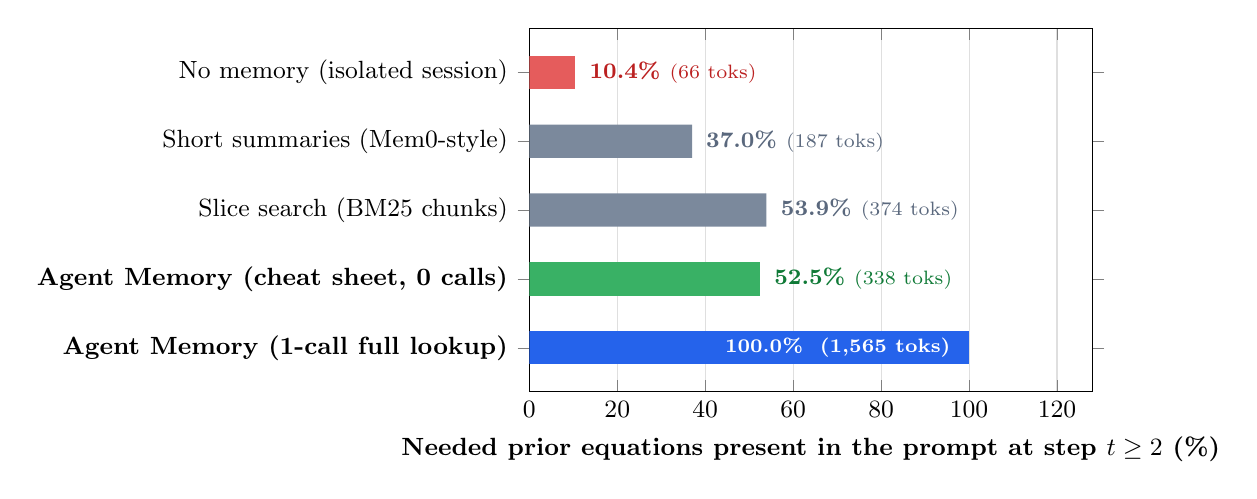
\begin{tikzpicture}
\begin{axis}[
  xbar,width=0.72\textwidth,height=6.2cm,
  xmin=0,xmax=128,
  xlabel={Needed prior equations present in the prompt at step $t \ge 2$ (\%)},
  symbolic y coords={r1,r2,r3,r4,r5},
  ytick={r1,r2,r3,r4,r5},
  yticklabels={
    {No memory (isolated session)},
    {Short summaries (Mem0-style)},
    {Slice search (BM25 chunks)},
    {\textbf{Agent Memory (cheat sheet, 0 calls)}},
    {\textbf{Agent Memory (1-call full lookup)}}
  },
  y dir=reverse,
  bar width=12pt,bar shift=0pt,enlarge y limits=0.16,
  tick label style={font=\small},
  label style={font=\small\bfseries},
  xmajorgrids,grid style={gray!25}]
\addplot[fill=amred!75,draw=none] coordinates {(10.4,r1)};
\addplot[fill=amgray!85,draw=none] coordinates {(37.0,r2) (53.9,r3)};
\addplot[fill=amgreen!85,draw=none] coordinates {(52.5,r4)};
\addplot[fill=amblue,draw=none] coordinates {(100.0,r5)};

\node[anchor=west,font=\footnotesize\bfseries,text=amred!85!black] at (axis cs:11.5,r1) {10.4\% \normalfont\scriptsize(66 toks)};
\node[anchor=west,font=\footnotesize\bfseries,text=amgray!90!black] at (axis cs:38.0,r2) {37.0\% \normalfont\scriptsize(187 toks)};
\node[anchor=west,font=\footnotesize\bfseries,text=amgray!90!black] at (axis cs:55.0,r3) {53.9\% \normalfont\scriptsize(374 toks)};
\node[anchor=west,font=\footnotesize\bfseries,text=amgreen!75!black] at (axis cs:53.5,r4) {52.5\% \normalfont\scriptsize(338 toks)};
\node[anchor=east,font=\scriptsize\bfseries,text=white] at (axis cs:98,r5) {100.0\% \ (1,565 toks)};
\end{axis}
\end{tikzpicture}
\caption{Equation retention across all 20 physics papers (66 dependent subtasks). Short summaries lose nearly two-thirds of the math (37.0\% kept). Fixed-slice search loses nearly half (53.9\%). Agent Memory's 1{,}200-character cheat sheet matches slice search with \emph{zero} lookups (52.5\%, green bar), and adding a single full lookup keeps \textbf{100.0\%} of needed equations (blue bar).}
\label{fig:recall}
\end{figure}

\subsection*{Finding 2: On the official benchmark model (\texttt{gpt-5-mini}), Agent Memory ranks \#1}

To make a strict apples-to-apples comparison against the published ICML 2026 leaderboard, we ran all 20 papers using the benchmark's exact official model (\texttt{gpt-5-mini}) and official LLM equivalence judge (\texttt{MathEnvironment.judge()}).

On Step 1 alone---before any memory system is even used---\texttt{gpt-5-mini} only solves \textbf{12 out of 20 problems (60\%)} due to single-step algebra errors. That 12-problem mark is the ceiling of what a perfect memory system could preserve for this model (Figure~\ref{fig:mini}).

\begin{figure}[H]
\centering
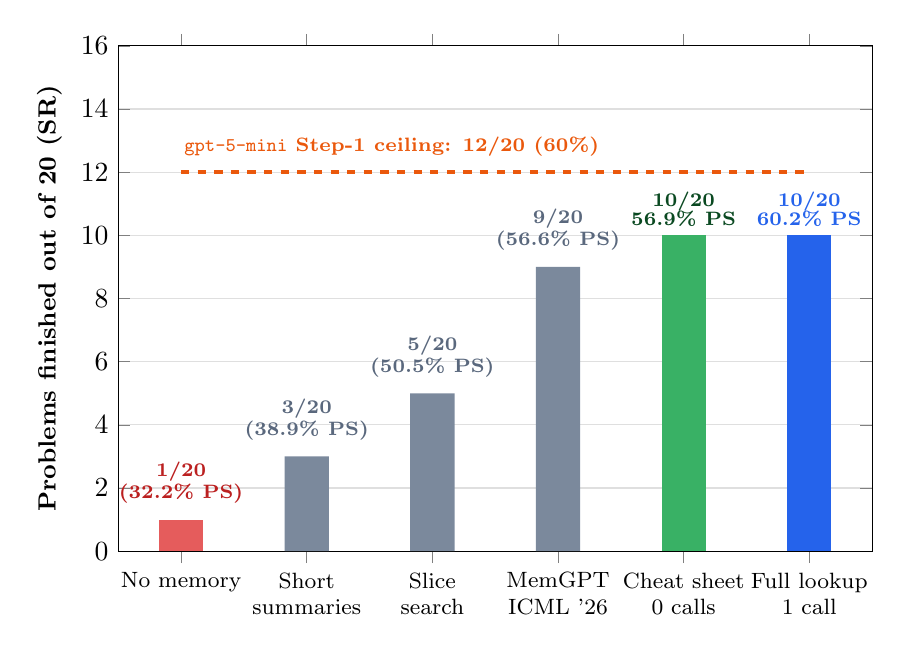
\begin{tikzpicture}
\begin{axis}[
  ybar,width=0.92\textwidth,height=8.0cm,bar width=16pt,bar shift=0pt,
  ymin=0,ymax=16,clip=false,ylabel={Problems finished out of 20 (SR)},
  symbolic x coords={m1,m2,m3,m4,m5,m6},
  xtick={m1,m2,m3,m4,m5,m6},
  xticklabels={
    {No memory},
    {Short\\summaries},
    {Slice\\search},
    {MemGPT\\ICML '26},
    {Cheat sheet\\0 calls},
    {Full lookup\\1 call}
  },
  x tick label style={font=\footnotesize,align=center},
  label style={font=\small\bfseries},
  ymajorgrids,grid style={gray!25}]
\addplot[fill=amred!75,draw=none] coordinates {(m1,1)};
\addplot[fill=amgray!85,draw=none] coordinates {(m2,3) (m3,5) (m4,9)};
\addplot[fill=amgreen!85,draw=none] coordinates {(m5,10)};
\addplot[fill=amblue,draw=none] coordinates {(m6,10)};

\draw[amorange,very thick,dashed] (axis cs:m1,12) -- (axis cs:m6,12);
\node[anchor=south west,font=\scriptsize\bfseries,text=amorange,inner sep=1pt] at (axis cs:m1,12.4) {\texttt{gpt-5-mini} Step-1 ceiling: 12/20 (60\%)};

\node[anchor=south,font=\scriptsize\bfseries,align=center,text=amred!85!black] at (axis cs:m1,1.2) {1/20\\(32.2\% PS)};
\node[anchor=south,font=\scriptsize\bfseries,align=center,text=amgray!90!black] at (axis cs:m2,3.2) {3/20\\(38.9\% PS)};
\node[anchor=south,font=\scriptsize\bfseries,align=center,text=amgray!90!black] at (axis cs:m3,5.2) {5/20\\(50.5\% PS)};
\node[anchor=south,font=\scriptsize\bfseries,align=center,text=amgray!90!black] at (axis cs:m4,9.2) {9/20\\(56.6\% PS)};
\node[anchor=south,font=\scriptsize\bfseries,align=center,text=amgreen!45!black,inner sep=0pt] at (axis cs:m5,10.25) {10/20\\[-1pt]56.9\% PS};
\node[anchor=south,font=\scriptsize\bfseries,align=center,text=amblue,inner sep=0pt] at (axis cs:m6,10.25) {10/20\\[-1pt]60.2\% PS};
\end{axis}
\end{tikzpicture}
\caption{Results across all 20 papers using the official \texttt{gpt-5-mini} solver + LLM judge. Without memory, performance collapses from 12/20 on Step 1 down to 1/20 at the end. Agent Memory finishes \textbf{10 of the 12 solvable problems (50.0\% SR; 56.9\% PS for cheat sheet only in green, 60.2\% PS for full lookup in blue)}, beating all published external memory systems.}
\label{fig:mini}
\end{figure}

\subsection*{Finding 3: With a stronger AI (\texttt{gpt-5.6-sol}), Agent Memory finishes 20 out of 20}

To separate memory failures from algebra mistakes, we ran all 20 papers (86 steps) with a stronger solver (\texttt{gpt-5.6-sol}) that gets \textbf{all 20 first steps right (100\%)}. Now any failure on Steps $2\dots 12$ is purely a memory failure (Figure~\ref{fig:sol}).

\begin{figure}[H]
\centering
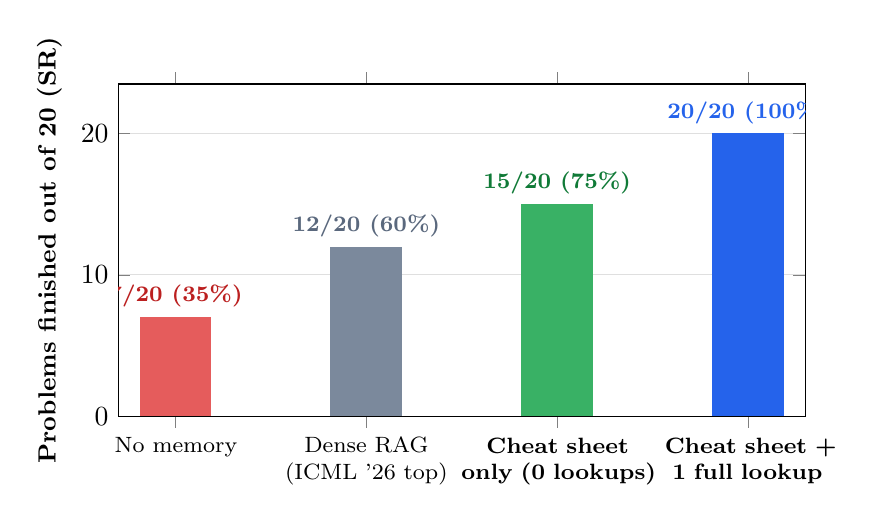
\begin{tikzpicture}
\begin{axis}[
  ybar,width=0.85\textwidth,height=5.8cm,bar width=26pt,bar shift=0pt,
  ymin=0,ymax=23.5,ylabel={Problems finished out of 20 (SR)},
  symbolic x coords={s1,s2,s3,s4},
  xtick={s1,s2,s3,s4},
  xticklabels={
    {No memory},
    {Dense RAG (ICML '26 top)},
    {\textbf{Cheat sheet only (0 lookups)}},
    {\textbf{Cheat sheet + 1 full lookup}}
  },
  x tick label style={font=\footnotesize,align=center,text width=2.8cm},
  label style={font=\small\bfseries},
  ymajorgrids,grid style={gray!25}]
\addplot[fill=amred!75,draw=none] coordinates {(s1,7)};
\addplot[fill=amgray!85,draw=none] coordinates {(s2,12)};
\addplot[fill=amgreen!85,draw=none] coordinates {(s3,15)};
\addplot[fill=amblue,draw=none] coordinates {(s4,20)};

\node[anchor=south,font=\footnotesize\bfseries,text=amred!85!black] at (axis cs:s1,7) {7/20 (35\%)};
\node[anchor=south,font=\footnotesize\bfseries,text=amgray!90!black] at (axis cs:s2,12) {12/20 (60\%)};
\node[anchor=south,font=\footnotesize\bfseries,text=amgreen!75!black] at (axis cs:s3,15) {15/20 (75\%)};
\node[anchor=south,font=\footnotesize\bfseries,text=amblue] at (axis cs:s4,20) {20/20 (100\%)};
\end{axis}
\end{tikzpicture}
\caption{With \texttt{gpt-5.6-sol}, the 1{,}200-character cheat sheet alone finishes \textbf{15 of 20 papers (75.0\% SR, 85.8\% PS, green)} with zero tool calls ($\sim 197$ tokens/turn), and adding one full lookup finishes \textbf{all 20 papers (100.0\% SR, 86/86 subtasks solved, blue)}.}
\label{fig:sol}
\end{figure}

\subsection*{Finding 4: The longer the chain, the bigger the gap}

Figure~\ref{fig:depth} tracks accuracy step by step from Session 1 to Session 12. Without memory, even the strong model drops from 100\% at Step 1 to 45\% at Step 2 and 0\% after Step 6. The one-paragraph cheat sheet holds up well through Step 8 (66.7\%), and the one-request full lookup stays at \textbf{100\% all the way to Step 12}.

\begin{figure}[H]
\centering
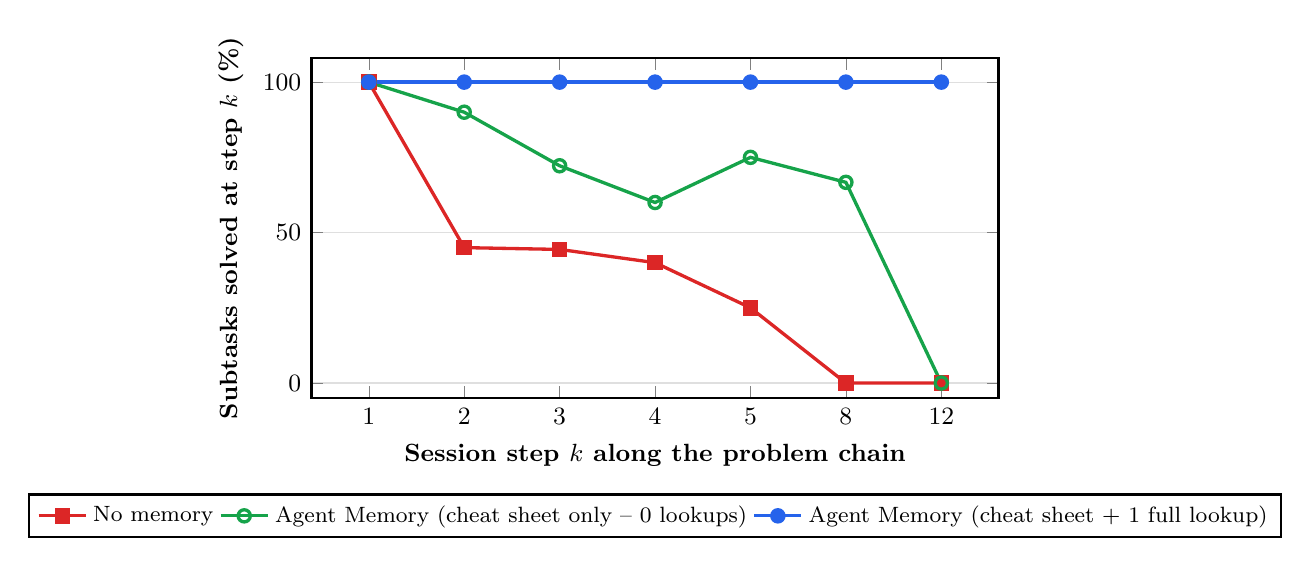
\begin{tikzpicture}
\begin{axis}[
  width=0.85\textwidth,height=5.9cm,
  xlabel={Session step $k$ along the problem chain},ylabel={Subtasks solved at step $k$ (\%)},
  symbolic x coords={1,2,3,4,5,8,12},
  xtick={1,2,3,4,5,8,12},
  ymin=-5,ymax=108,
  tick label style={font=\small},
  label style={font=\small\bfseries},
  legend style={at={(0.5,-0.28)},anchor=north,legend columns=3,font=\footnotesize},
  ymajorgrids,grid style={gray!25},mark size=2.2pt,thick]
\addplot[color=amred,mark=square*,very thick] coordinates {(1,100)(2,45)(3,44.4)(4,40)(5,25)(8,0)(12,0)};
\addplot[color=amgreen,mark=o,very thick] coordinates {(1,100)(2,90)(3,72.2)(4,60)(5,75)(8,66.7)(12,0)};
\addplot[color=amblue,mark=*,very thick] coordinates {(1,100)(2,100)(3,100)(4,100)(5,100)(8,100)(12,100)};
\legend{No memory,Agent Memory (cheat sheet only -- 0 lookups),Agent Memory (cheat sheet + 1 full lookup)}
\end{axis}
\end{tikzpicture}
\caption{Accuracy by session depth $k$ with \texttt{gpt-5.6-sol}. Without memory (red) accuracy collapses as chains get deeper; the 1{,}200-char cheat sheet (green) carries the agent through medium chains; one full lookup (blue) prevents decay through Step 12.}
\label{fig:depth}
\end{figure}

% ---------------------------------------------------------------
\section{What this does and does not show}

To keep our claims honest:
\begin{itemize}[itemsep=2pt,leftmargin=1.5em]
  \item \textbf{Evaluated on formal physics derivations.} Our live benchmark covers all 20 papers (86 subtasks) of MemoryArena's physics split (\texttt{formal\_reasoning\_phys}). While our adapter plugs directly into the other MemoryArena splits (math, CS, shopping, travel, search), we have only run the physics split so far.
  \item \textbf{Why we report two AI models.} On the benchmark's standard model (\texttt{gpt-5-mini}), Agent Memory achieves \textbf{50.0\% SR and 60.2\% PS}---beating MemGPT (45\% SR), Mem0 (25\% SR), and GPT-5.1-mini Long Context (45\% SR / 60\% PS), while sitting right at \texttt{gpt-5-mini}'s 60\% single-step math ceiling. Running \texttt{gpt-5.6-sol} (100\% SR / 100\% PS) shows what happens when single-step algebra errors are removed.
  \item \textbf{Deep chains need the full lookup.} A 1{,}200-character paragraph ($\sim 200$ tokens) solves 75\% of papers with zero tool calls, but chains of 8--12 equations require calling \texttt{memory\_find(..., full=True)} ($\sim 968$--$1{,}435$ tokens).
\end{itemize}

\section{Conclusion}

Memory for AI assistants does not need to rely on lossy AI summaries or arbitrary text slicing. By saving complete notes as Git snapshots, compiling a deterministic 1{,}200-character cheat sheet every turn, folding finished steps into consecutive summaries or algebraic rules, and supporting one-call symbol-aware full lookup, Agent Memory preserves 100\% of the underlying math and lets capable agents finish long, multi-session tasks without losing the thread.

\begin{glossarybox}
\textbf{Glossary.}
\textbf{Agent:} an AI assistant that works on a task across many steps and tool calls.
\textbf{Session:} one work period; each new session starts with a fresh context window.
\textbf{Long context:} feeding the entire past conversation transcript into every prompt.
\textbf{RAG (Retrieval-Augmented Generation):} slicing past text into chunks and searching for matches.
\textbf{FTS5 \& RRF:} SQLite's fast full-text keyword search, combined with semantic search via Reciprocal Rank Fusion.
\textbf{Git \& SHA-256:} version-control snapshots and cryptographic file fingerprints used to detect when files change.
\end{glossarybox}

\end{document}
